\documentclass[12pt,b5paper]{ltjsarticle}

%\usepackage[margin=15truemm, top=5truemm, bottom=5truemm]{geometry}
\usepackage[margin=15truemm]{geometry}

\usepackage{amsmath,amssymb}
%\pagestyle{headings}
\pagestyle{empty}

%\usepackage{listings,url}
%\renewcommand{\theenumi}{(\arabic{enumi})}

\usepackage{graphicx}

\usepackage{tikz}
\usetikzlibrary {arrows.meta}
\usepackage{wrapfig}	% required for `\wrapfigure' (yatex added)
\usepackage{bm}	% required for `\bm' (yatex added)

% ルビを振る
%\usepackage{luatexja-ruby}	% required for `\ruby'

%% 核Ker 像Im Hom を定義
%\newcommand{\Img}{\mathop{\mathrm{Im}}\nolimits}
%\newcommand{\Ker}{\mathop{\mathrm{Ker}}\nolimits}
%\newcommand{\Hom}{\mathop{\mathrm{Hom}}\nolimits}

\begin{document}

\begin{equation}
 \bm{f}=
  \begin{pmatrix}
   f_1(x,y)\\
   f_2(x,y)
  \end{pmatrix}
\end{equation}

\hrulefill

開区間$I_{\alpha,\beta}=(\alpha,\beta),\,I_{\gamma,\delta}=(\gamma,\delta)$
の直積上の関数$F$を次のように定める。
\begin{equation}
 F: I_{\alpha,\beta} \times I_{\gamma,\delta} \times I_{\gamma,\delta}
  \to \mathbb{R},
  \quad (x,u,v) \mapsto \int_{u}^{v}f_2(x,y)\mathrm{d}y
\end{equation}

ベクトル値関数$\bm{g}$を次のように定める。
\begin{equation}
 \bm{g}: I_{\alpha,\beta} \to \mathbb{R}^3,
  \quad x \mapsto \begin{pmatrix}x\\\varphi(x)\\\psi(x)\end{pmatrix}
\end{equation}

この時、合成関数$F\circ \bm{g}$は次のようになる。
\begin{equation}
 F\circ\bm{g}(x) =F(\bm{g}(x))
  =F(x,\varphi(x),\psi(x))
  =\int_{\varphi(x)}^{\psi(x)}f_2(x,y)\mathrm{d}y
\end{equation}

縦線集合$D_{ij}$を次のような集合とする。
\begin{equation}
 D_{ij} = \{ (x,y)\in\mathbb{R}^2 \mid a\leq x\leq b ,\, \varphi(x)\leq y\leq \psi(x)\}
\end{equation}


\begin{center}
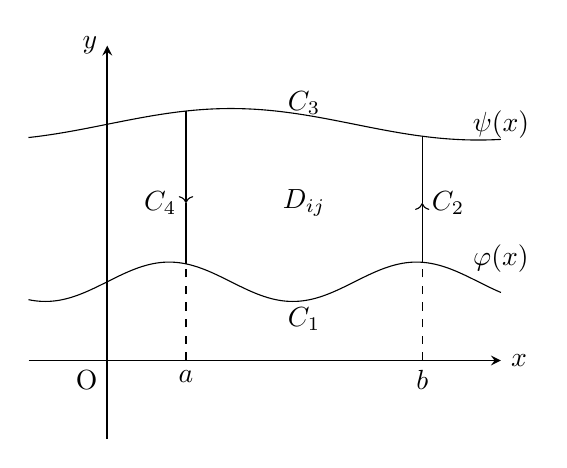
\begin{tikzpicture}[scale=1,samples=300]

\draw[->,>=stealth,semithick] (-1,0)--(5,0) node[right]{$x$}; %x軸
\draw[->,>=stealth,semithick] (0,-1)--(0,4) node[left]{$y$}; %y軸
\draw (0,0) node[below left]{O}; %原点

\draw[thin,domain=-1:5] plot(\x,{1/4*sin(2*\x r)+1});
\draw (5,1) node[above]{$\varphi(x)$};
\draw[thin,domain=-1:5] plot(\x,{1/5*sin(\x r)+3});
\draw (5,3) node{$\psi(x)$};

%\draw[dashed] (0,2)node[left]{2}--(pi,2)--(pi,0)node[below]{$\pi$};

\draw[dashed] (1,0) node [below] {$a$} -- (1,{1/5*sin(1 r)+3});
\draw[->] (1,{1/5*sin(1 r)+3})--(1,2);
\draw (1,2)--(1,{1/4*sin(2*1 r)+1});
\node[left] at (1,2) {$C_4$};

\draw[dashed] (4,0) node [below] {$b$}--(4,{1/4*sin(2*4 r)+1});
\draw[<-] (4,2)--(4,{1/4*sin(2*4 r)+1});
\draw (4,{1/5*sin(4 r)+3})--(4,2);
\node[right] at (4,2) {$C_2$};


\node at (2.5,2) {$D_{ij}$};

\node[below] at (2.5,0.8) {$C_{1}$};
\node[above] at (2.5,3) {$C_{3}$};

\end{tikzpicture}
\end{center}

この時、次の式を示せ。
\begin{enumerate}
 \item
     \begin{equation}
      \int_{C_1}\bm{f}
       = \int_{a}^{b}(f_1(x,\varphi(x)) + f_2(x,\varphi(x))\varphi^{\prime}(x)))\mathrm{d}x
     \end{equation}
 \item
     \begin{equation}
      \int_{C_2}\bm{f}
       = \int_{\varphi(b)}^{\psi(b)}f_2(b,y)\mathrm{d}y
     \end{equation}
 \item
     \begin{equation}
      \int_{C_3}\bm{f}
       = - \int_{a}^{b}(f_1(x,\psi(x)) + f_2(x,\psi(x))\psi^{\prime}(x))\mathrm{d}x
     \end{equation}
 \item
     \begin{equation}
      \int_{C_4}\bm{f}
       = -\int_{\varphi(a)}^{\psi(a)}f_2(a,y)\mathrm{d}y
     \end{equation}
\end{enumerate}

\dotfill

\begin{enumerate}
 \item
      曲線$C_1$は点$(a,\varphi(a))$から点$(b,\varphi(b))$を結ぶ曲線で
      この間の点は$(t,\varphi(t))$である。
%      $t$は$a$から$b$へ変化する媒介変数である。
      そこで、
%       $\begin{pmatrix}f_1(x,y)\end{pmatrix}$
      $y=\varphi(x)$として、
      $\bm{f}=\bm{f}(x,y)=\bm{f}(x,\varphi(x))$
      を$C_1$に沿って積分する。

      $y$は$x$を媒介変数にもつ関数であるので、
      $\begin{pmatrix}\mathrm{d}x\\\mathrm{d}y\end{pmatrix}$
      を
      $\begin{pmatrix}\frac{\mathrm{d}x}{\mathrm{d}x}\\\frac{\mathrm{d}y}{\mathrm{d}x}\end{pmatrix}\mathrm{d}x$
      に置き換える。

      これにより$\bm{f}$との内積が次のようになる。
      \begin{equation}
       \bm{f}\cdot \begin{pmatrix}\frac{\mathrm{d}x}{\mathrm{d}x}\\\frac{\mathrm{d}y}{\mathrm{d}x}\end{pmatrix}
       = \begin{pmatrix}f_1(x,y)\\f_2(x,y)\end{pmatrix}
      \cdot \begin{pmatrix}1\\\frac{\mathrm{d}y}{\mathrm{d}x}\end{pmatrix}
      = f_1(x,y)+f_2(x,y)\frac{\mathrm{d}y}{\mathrm{d}x}
      \end{equation}

      この式に$y=\varphi(x)$を代入すると次の式を得る。

      \begin{align}
       \int_{C_1}\bm{f}
       =& \int_{a}^{b}\bm{f}
             \cdot\begin{pmatrix}\frac{\mathrm{d}x}{\mathrm{d}x}\\\frac{\mathrm{d}\varphi(x)}{\mathrm{d}x}\end{pmatrix}\mathrm{d}x\\
       =& \int_{a}^{b}
       \left(f_1(x,\varphi(x)) + f_2(x,\varphi(x))\varphi^{\prime}(x)\right)\mathrm{d}x
      \end{align}


 \item
      $C_2$は点$(b,\varphi(b))$から点$(b,\psi(b))$を結ぶ線分である。
      この為、$C_2$上では$\bm{f}=\bm{f}(b,y)$であり、$y$が$\varphi(b)$から$\psi(b)$に変化し、
      $x$は定数$b$の値を取る。

      $x$の値は$b$で変化せず、$y$だけが変化するので、
      \begin{equation}
       \bm{f}\cdot \begin{pmatrix}\frac{\mathrm{d}b}{\mathrm{d}y}\\\frac{\mathrm{d}y}{\mathrm{d}y}\end{pmatrix}
       = \begin{pmatrix}f_1(x,y)\\f_2(x,y)\end{pmatrix}
      \cdot \begin{pmatrix}0\\1\end{pmatrix}
      = f_2(x,y)
      \end{equation}
      となる。

      この為、$C_2$上の積分は次のようになる。
      \begin{align}
      \int_{C_2}\bm{f}
       =& \int_{\varphi(b)}^{\psi(b)}\bm{f}
             \cdot\begin{pmatrix}\frac{\mathrm{d}b}{\mathrm{d}y}\\\frac{\mathrm{d}y}{\mathrm{d}y}\end{pmatrix}\mathrm{d}y\\
       =& \int_{\varphi(b)}^{\psi(b)}f_2(b,y)\mathrm{d}y
      \end{align}

 \item
      曲線$C_3$は点$(b,\psi(b))$から点$(a,\psi(a))$を結ぶ曲線である。
      $C_1$の時と同様の手順で次のように求まる。
      \begin{align}
       \int_{C_3}\bm{f}
       =& \int_{b}^{a}\bm{f}
             \cdot\begin{pmatrix}\frac{\mathrm{d}x}{\mathrm{d}x}\\\frac{\mathrm{d}\psi(x)}{\mathrm{d}x}\end{pmatrix}\mathrm{d}x\\
       =& \int_{b}^{a}
       \left(f_1(x,\psi(x)) + f_2(x,\psi(x))\psi^{\prime}(x)\right)\mathrm{d}x\\
       =& - \int_{a}^{b}(f_1(x,\psi(x)) + f_2(x,\psi(x))\psi^{\prime}(x))\mathrm{d}x
      \end{align}

 \item
      $C_4$は点$(a,\psi(a))$から点$(a,\varphi(a))$を結ぶ線分である。
      $C_2$の場合と同様の手順で求まる。
      \begin{align}
      \int_{C_4}\bm{f}
       =& \int_{\psi(a)}^{\varphi(a)}\bm{f}
             \cdot\begin{pmatrix}\frac{\mathrm{d}a}{\mathrm{d}y}\\\frac{\mathrm{d}y}{\mathrm{d}y}\end{pmatrix}\mathrm{d}y\\
       =& \int_{\psi(a)}^{\varphi(a)}f_2(a,y)\mathrm{d}y\\
       =& -\int_{\varphi(a)}^{\psi(a)}f_2(a,y)\mathrm{d}y
      \end{align}


\end{enumerate}
\hrulefill


\end{document}
